\documentclass[12pt,a4paper]{article}
% =============================================================================
% PAPER A — A austeridade educacional se autofinancia?
% Efeito Laffer dinâmico do gasto público em educação num DSGE fiscal
% =============================================================================
\usepackage[utf8]{inputenc}
\usepackage[T1]{fontenc}
\usepackage[brazil]{babel}
\usepackage{mathptmx}
\usepackage{geometry}
\geometry{a4paper,left=1.8cm,right=1.8cm,top=2cm,bottom=2cm}
\usepackage{setspace}
\singlespacing
\usepackage{graphicx}
\usepackage{float}
\usepackage{booktabs}
\usepackage{array}
\usepackage{tabularx}
\usepackage{caption}
\usepackage{amsmath,amssymb}
\usepackage{enumitem}
\usepackage[round,authoryear]{natbib}
\bibliographystyle{plainnat}
\usepackage[colorlinks=true,linkcolor=black,citecolor=blue!50!black,urlcolor=blue!50!black]{hyperref}
\renewcommand{\tablename}{Tabela}
\renewcommand{\figurename}{Figura}
\renewcommand{\bibname}{Refer\^encias}
\captionsetup{font=small,labelfont=bf,justification=centering}
\newcolumntype{Y}{>{\arraybackslash}X}
\newcommand{\fonte}[1]{\captionsetup{font=scriptsize}\caption*{\footnotesize Fonte: #1}}
\newcommand{\Ee}{\mathbb{E}}

\title{\textbf{A Austeridade Educacional se Autofinancia?}\\[2pt]
\textbf{\large Efeito Laffer Din\^amico do Gasto P\'ublico em Educa\c{c}\~ao\\ num DSGE Fiscal com Capital Humano}}
\author{Valber Gregory Barbosa Costa Bezerra Santos\thanks{Universidade Federal de Alagoas (UFAL) -- Unidade Educacional de Penedo; Tribunal de Justi\c{c}a do Estado de Alagoas. E-mail: \texttt{valber.santos@penedo.ufal.br}. Para avalia\c{c}\~ao \`as cegas, suprimir esta nota.}}
\date{\today}

\begin{document}
\maketitle
\vspace{-0.5cm}
\begin{center}\small
\textbf{\'Area ANPEC:} 5 -- Economia do Setor P\'ublico (aderente \`a 4 -- Macroeconomia).\\
\textbf{JEL:} E62; H52; I28; O41; H63; E32.
\end{center}

\begin{abstract}
\noindent Cortes no gasto p\'ublico em educa\c{c}\~ao s\~ao usualmente avaliados pelo seu al\'ivio or\c{c}ament\'ario imediato. Este artigo mostra que essa contabilidade \'e ilus\'oria. Desenvolve-se um modelo din\^amico estoc\'astico de equil\'ibrio geral (DSGE) fiscal com capital f\'isico e humano, tributa\c{c}\~ao distorciva e gasto p\'ublico em educa\c{c}\~ao como insumo produtivo da acumula\c{c}\~ao de capital humano, resolvido por previs\~ao perfeita n\~ao linear com estado estacion\'ario terminal end\'ogeno. Simulam-se cortes permanentes de $1\%$, $5\%$, $10\%$ e $25\%$ e um cen\'ario de teto de gasto (EC 95/2016). Um corte permanente de $10\%$ reduz o produto de longo prazo em $3{,}4\%$ e imp\~oe perdas de bem-estar de at\'e $2{,}4\%$ do consumo permanente (corte de $25\%$); o multiplicador acumulado do gasto educacional sobre o produto supera a unidade. O resultado central \'e um \emph{efeito Laffer din\^amico da educa\c{c}\~ao}: como a arrecada\c{c}\~ao segue o produto ($T=\tau Y$), o corte corr\'oi a pr\'opria base tribut\'aria; em valor presente de 30 anos, at\'e $78\%$ da economia or\c{c}ament\'aria \'e revertida, com \emph{break-even} fiscal por volta do ano 33. A sensibilidade ao par\^ametro-chave $\phi$ (elasticidade do capital humano ao gasto) revela um \emph{limiar de autofinanciamento}: acima de $\phi\approx 0{,}45$, o corte perde dinheiro at\'e em valor presente. Conclui-se que a austeridade educacional \'e, em horizonte relevante, fiscalmente autodestrutiva.

\vspace{0.2cm}
\noindent\textbf{Palavras-chave:} gasto p\'ublico em educa\c{c}\~ao; capital humano; DSGE fiscal; efeito Laffer; multiplicador fiscal; austeridade.
\end{abstract}
\noindent\textbf{Abstract.} Cuts to public education spending are usually judged by their immediate budget relief. This paper shows that accounting to be illusory. A fiscal DSGE with physical and human capital, distortionary taxation and public education spending as a productive input into human-capital accumulation is solved by nonlinear perfect foresight with an endogenous terminal steady state. A permanent $10\%$ cut lowers long-run output by $3.4\%$ and imposes welfare losses up to $2.4\%$ of permanent consumption; the cumulative output multiplier of education spending exceeds one. The central result is a \emph{dynamic education Laffer effect}: since revenue tracks output, the cut erodes its own tax base, undoing up to $78\%$ of the budget saving in 30-year present value (fiscal break-even around year 33). Sensitivity to the key parameter $\phi$ reveals a \emph{self-financing threshold}: above $\phi\approx 0.45$ the cut loses money even in present value. \textbf{Keywords:} public education spending; human capital; fiscal DSGE; Laffer effect; fiscal multiplier. \textbf{JEL:} E62; H52; I28; O41; H63; E32.

% =============================================================================
\section{Introdu\c{c}\~ao}
% =============================================================================
A avalia\c{c}\~ao de pol\'iticas de conten\c{c}\~ao or\c{c}ament\'aria costuma restringir-se ao seu custo fiscal imediato. No caso da educa\c{c}\~ao, essa \'otica \'e particularmente enganosa: o gasto educacional \'e um \emph{investimento} produtivo, que constr\'oi capital humano e, por essa via, produto, sal\'arios e -- crucialmente -- a pr\'opria base de arrecada\c{c}\~ao futura. Cortar educa\c{c}\~ao economiza recursos hoje, mas reduz a arrecada\c{c}\~ao amanh\~a. A quest\~ao central deste artigo \'e direta: \emph{um corte no gasto p\'ublico em educa\c{c}\~ao efetivamente economiza dinheiro p\'ublico?}

O tema \'e premente no Brasil ap\'os o Novo Regime Fiscal (Emenda Constitucional n.\ 95/2016), que limitou o crescimento real do gasto prim\'ario e pressionou despesas discricion\'arias \citep{rocha2017teto}, e diante de epis\'odios recorrentes de bloqueio ou conten\c{c}\~ao de repasses a universidades e institutos federais. A contribui\c{c}\~ao \'e tr\'iplice. \emph{Primeiro}, desenvolve-se um DSGE fiscal com capital humano financiado publicamente, na tradi\c{c}\~ao de \citet{uzawa1965}, \citet{lucas1988}, \citet{glommravikumar1992} e \citet{barro1990}, com o bloco fiscal de tributa\c{c}\~ao distorciva da gera\c{c}\~ao moderna \citep{leeper2010,drautzburguhlig2015}, resolvido por previs\~ao perfeita n\~ao linear. \emph{Segundo}, quantifica-se o \emph{custo fiscal l\'iquido} em R\$ de cortes de diferentes magnitudes, revelando um \emph{efeito Laffer din\^amico da educa\c{c}\~ao}: parcela substancial -- e crescente no tempo -- da ``economia'' \'e revertida pela menor arrecada\c{c}\~ao. \emph{Terceiro}, mede-se a sensibilidade desse efeito ao par\^ametro estrutural que governa a produtividade do gasto ($\phi$), identificando um \emph{limiar de autofinanciamento} acima do qual o corte perde dinheiro at\'e em valor presente.

O principal achado \'e que a austeridade educacional \'e, em horizonte relevante, fiscalmente autodestrutiva: o corte de curto prazo \'e progressivamente -- e, sob calibra\c{c}\~oes plaus\'iveis, integralmente -- anulado pela eros\~ao da base tribut\'aria, al\'em de impor perdas de produto e bem-estar.

% =============================================================================
\section{Revis\~ao de literatura}
% =============================================================================
A modelagem DSGE evoluiu dos ciclos reais \citep{kydlandprescott1982} \`a vers\~ao novo-keynesiana estimada \citep{smetswouters2007}, com m\'etodos sistematizados por \citet{schmittgrohe2004} e \citet{fvrr2016}. Blocos fiscais com tributa\c{c}\~ao distorciva e regras de gasto s\~ao tratados por \citet{galilv2007}, \citet{leeper2010} e \citet{drautzburguhlig2015}, que mostram que a composi\c{c}\~ao do gasto \'e determinante de primeira ordem dos multiplicadores. A literatura de capital p\'ublico produtivo \citep{aschauer1989,bomligthart2014,leducwilson2013} estima a elasticidade do produto ao capital p\'ublico -- base para calibrar o canal produtivo aqui empregado, agora aplicado \`a forma\c{c}\~ao de capital humano. O papel do gasto p\'ublico em educa\c{c}\~ao sobre crescimento \'e formalizado por \citet{glommravikumar1992} e documentado por \citet{blankenausimpson2004} e \citet{blankenau2007}; \citet{manuelliseshadri2014} enfatizam o canal de qualidade do capital humano. A refer\^encia de calibra\c{c}\~ao brasileira vem do SAMBA \citep{castro2015samba} e dos DSGE fiscais de \citet{vereda2010} e \citet{cavalcantivereda2015}. O modelo aqui proposto fecha a ponte entre os modelos de educa\c{c}\~ao e crescimento e os DSGE fiscais, colocando o gasto educacional como insumo produtivo da acumula\c{c}\~ao de capital humano.

% =============================================================================
\section{O modelo}\label{sec:modelo}
% =============================================================================
\subsection{Fam\'ilias, firmas e capital humano}
Uma fam\'ilia representativa maximiza $\Ee_0 \sum_{t=0}^{\infty} \beta^t [\ln C_t + \theta \ln(1 - L_t)]$ sujeita a
$C_t + K_{t+1} - (1-\delta_k)K_t = (1-\tau)(w_t H_t L_t + r_t K_t) + \mathit{Tr}_t$,
gerando a equa\c{c}\~ao de Euler e a oferta de trabalho:
\begin{align}
\tfrac{1}{C_t} &= \beta\,\Ee_t\!\left[\tfrac{1}{C_{t+1}}\big((1-\tau)\,r_{t+1} + 1 - \delta_k\big)\right], \label{eq:euler}\\
\tfrac{\theta}{1-L_t} &= \tfrac{1}{C_t}(1-\tau)\,w_t H_t. \label{eq:labor}
\end{align}
A produ\c{c}\~ao \'e $Y_t = K_t^{\alpha}(H_t L_t)^{1-\alpha}$, com $r_t=\alpha Y_t/K_t$ e $w_t=(1-\alpha)Y_t/(H_tL_t)$. O ingrediente central \'e a lei de movimento do capital humano com retornos decrescentes ao gasto:
\begin{equation}\label{eq:lomh}
H_{t+1} = (1-\delta_h)H_t + A\,(G^e_t)^{\phi}, \qquad 0<\phi<1,
\end{equation}
em que $\phi$ \'e a elasticidade de longo prazo do capital humano ao gasto p\'ublico. O governo opera com or\c{c}amento equilibrado, $\tau Y_t = G^e_t + \mathit{Tr}_t$, com arrecada\c{c}\~ao $T_t\equiv\tau Y_t$, e a restri\c{c}\~ao de recursos \'e $C_t + [K_{t+1}-(1-\delta_k)K_t] + G^e_t = Y_t$. O mecanismo fiscal fundamental \'e que a arrecada\c{c}\~ao \'e proporcional ao produto: reduzir $G^e$ deprime $H$, logo $Y$, logo $T$.

\subsection{Calibra\c{c}\~ao e solu\c{c}\~ao}
A calibra\c{c}\~ao (Tabela~\ref{tab:par}), anual, segue a literatura DSGE brasileira. O valor de refer\^encia $\phi=0{,}30$ situa-se na faixa das estimativas de produtividade do gasto p\'ublico produtivo \citep{bomligthart2014}; a se\c{c}\~ao de sensibilidade explora todo o intervalo $[0{,}15;0{,}45]$. A carga tribut\'aria efetiva $\tau=0{,}33$ reflete a raz\~ao carga/PIB. A transi\c{c}\~ao \'e resolvida por previs\~ao perfeita n\~ao linear (\emph{stacked-time} Newton) em 220 per\'iodos, com \emph{estado estacion\'ario terminal end\'ogeno} (solu\c{c}\~ao fechada para o n\'ivel de gasto p\'os-choque, Ap\^endice~\ref{ap:ss}), o que \'e essencial para cortes permanentes. A solu\c{c}\~ao converge com res\'iduo da ordem de $10^{-15}$.

\begin{table}[H]
\centering
\caption{Calibra\c{c}\~ao do modelo}
\label{tab:par}
\small
\begin{tabular}{cll}
\toprule
Parâmetro & Valor & Interpretação \\
\midrule
$\alpha$ & 0,40 & Participação do capital físico na produção \\
$\beta$ & 0,96 & Fator de desconto intertemporal (anual) \\
$\delta_k$ & 0,10 & Depreciação do capital físico \\
$\delta_h$ & 0,04 & Depreciação do capital humano \\
$\tau$ & 0,33 & Carga tributária efetiva (\% do PIB) \\
$\theta$ & 1,75 & Peso do lazer na utilidade \\
$\phi$ & 0,30 & Elasticidade do capital humano ao gasto público \\
$g_e$ & 0,05 & Gasto público em educação / PIB no EE \\
$\rho_G$ & 0,90 & Persistência do choque fiscal (transitório) \\
$A$ & 0,134 & Produtividade da tecnologia educacional (calibrada) \\
\bottomrule
\end{tabular}

\fonte{Elabora\c{c}\~ao pr\'opria; refer\^encia a \citet{castro2015samba} e \citet{cavalcantivereda2015}.}
\end{table}

% =============================================================================
\section{Resultados I: a escala do preju\'izo}\label{sec:res1}
% =============================================================================
A Figura~\ref{fig:irf} apresenta as respostas a um corte de $1\%$, transit\'orio (AR(1)) e permanente; no permanente, o capital humano cai $0{,}30\%$ (exatamente $\phi\%$) e o produto $0{,}33\%$, com o investimento liderando a queda inicial. A Tabela~\ref{tab:irf} detalha as perdas acumuladas.

\begin{figure}[H]
\centering
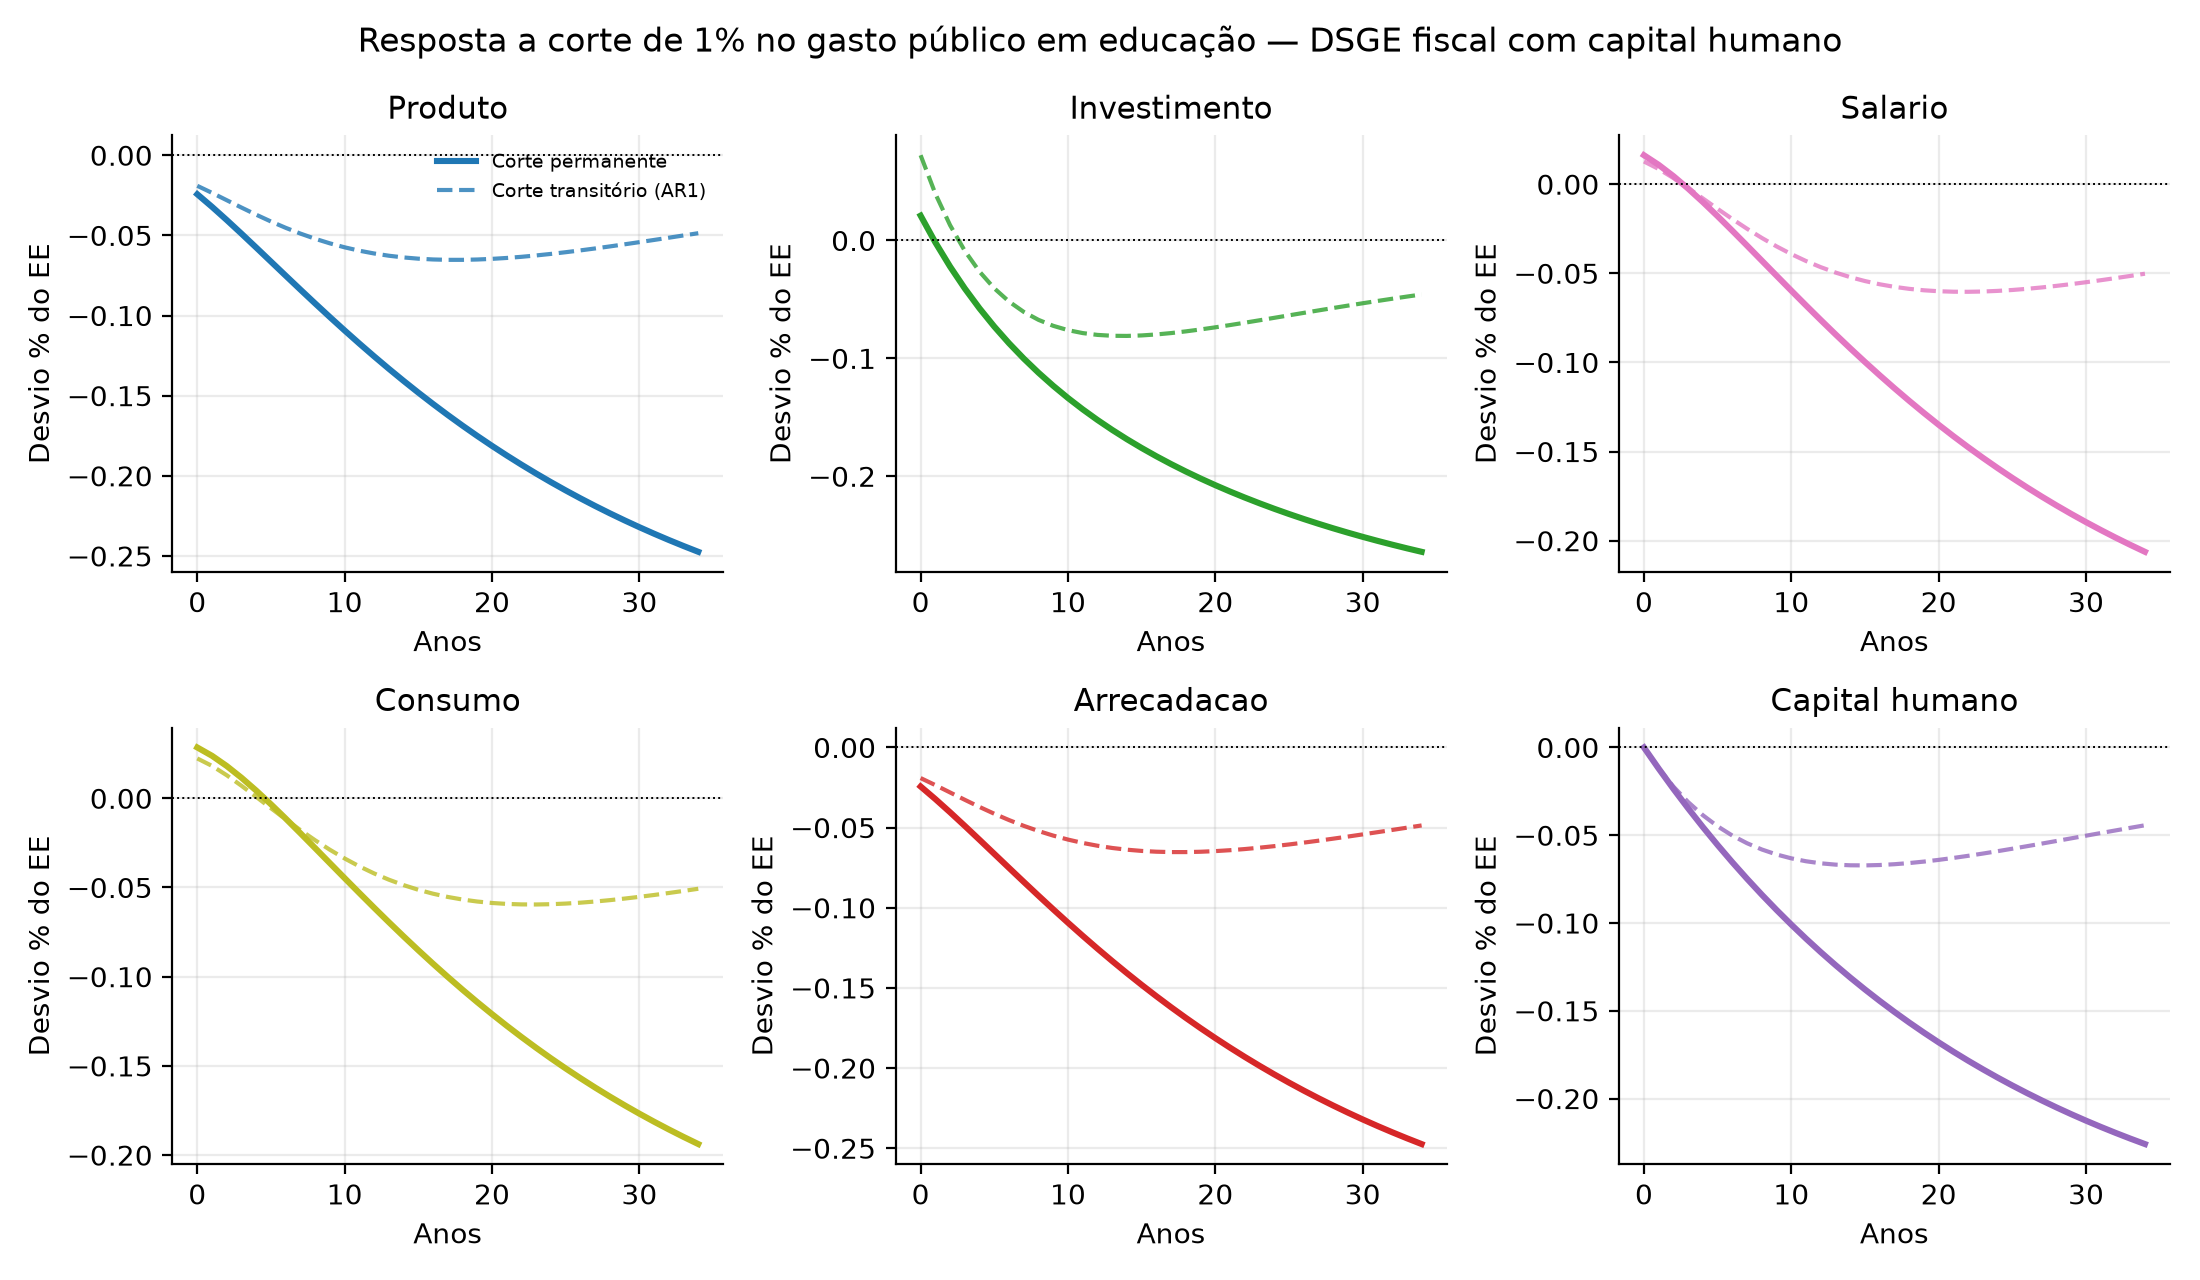
\includegraphics[width=0.85\textwidth]{figures/irf_corte_educacao.png}
\caption{Resposta a corte de $1\%$: permanente (cheia) e transit\'orio (tracejada)}
\label{fig:irf}
\fonte{Simula\c{c}\~ao DSGE.}
\end{figure}

\begin{table}[H]
\centering
\caption{Resposta ao corte permanente de $1\%$ (desvios \% do EE e perdas acumuladas)}
\label{tab:irf}
\small
\begin{tabular}{lrrrr}
\toprule
Variável & Impacto (t=0) & 5 anos & Perda acum. 10a & Perda acum. 20a \\
\midrule
Produto & -0,024 & -0,066 & 0,497 & 1,283 \\
Investimento & 0,021 & -0,073 & 0,455 & 1,391 \\
Salario & 0,016 & -0,018 & 0,108 & 0,623 \\
Consumo & 0,028 & -0,003 & -0,010 & 0,424 \\
Arrecadacao & -0,024 & -0,066 & 0,497 & 1,283 \\
\bottomrule
\end{tabular}

\fonte{Elabora\c{c}\~ao pr\'opria.}
\end{table}

A Figura~\ref{fig:multi} e a Tabela~\ref{tab:cen} escalam o choque: as perdas de longo prazo crescem de forma quase proporcional -- um corte de $10\%$ reduz o produto em $3{,}4\%$ e o capital humano em $3{,}1\%$; um de $25\%$, em $9{,}1\%$ e $8{,}3\%$. O cen\'ario de teto de gasto (EC 95), com compress\~ao gradual de $-10\%$ em oito anos, produz deteriora\c{c}\~ao mais lenta, por\'em permanente (Figura~\ref{fig:traj}): a aus\^encia de ``salto'' inicial mascara um dano estrutural que se acumula por d\'ecadas.

\begin{figure}[H]
\centering
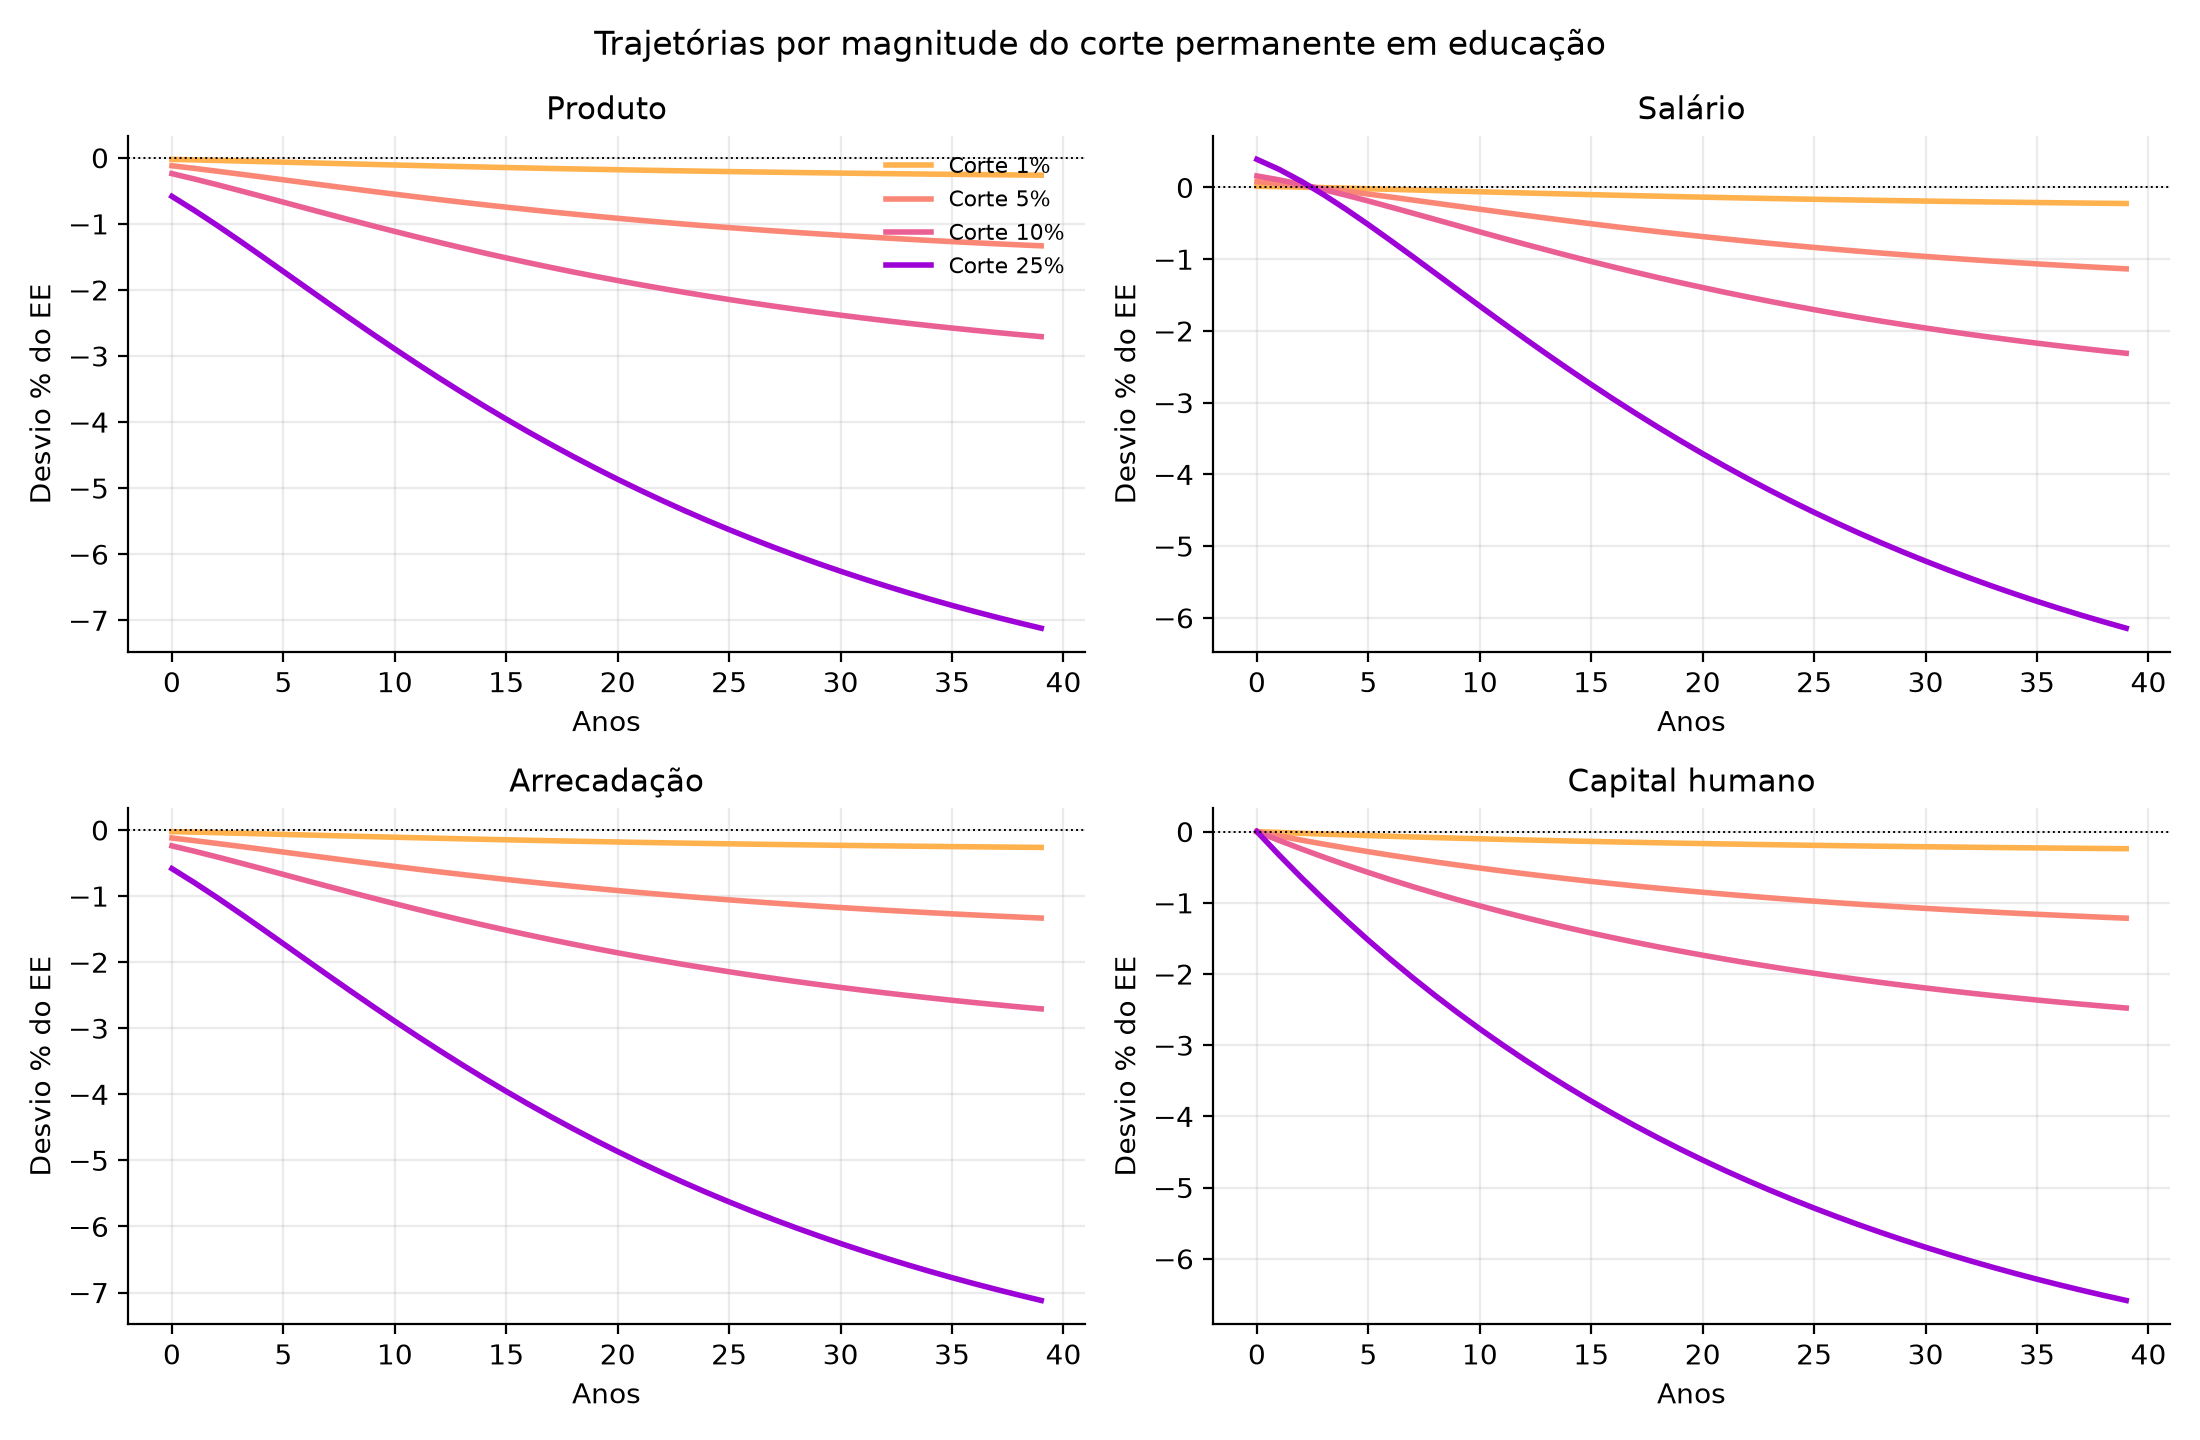
\includegraphics[width=\textwidth]{figures/irf_multi_corte.png}
\caption{Trajet\'orias por magnitude do corte permanente}
\label{fig:multi}
\fonte{Simula\c{c}\~ao DSGE.}
\end{figure}

\begin{table}[H]
\centering
\caption{Cen\'arios de corte: efeitos de longo prazo, bem-estar e multiplicador}
\label{tab:cen}
\small
\begin{tabular}{lrrrrrr}
\toprule
Corte & $\Delta H_{LP}$ & $\Delta Y_{LP}$ & $\Delta S_{LP}$ & $\Delta T_{LP}$ & Bem-estar & Mult.\ cum.\ 10a \\
 & (\%) & (\%) & (\%) & (\%) & (\% cons.) & \\
\midrule
1\% & -0,301 & -0,334 & -0,301 & -0,334 & 0,084 & 1,19 \\
5\% & -1,527 & -1,693 & -1,527 & -1,693 & 0,428 & 1,19 \\
10\% & -3,111 & -3,440 & -3,111 & -3,440 & 0,884 & 1,20 \\
25\% & -8,267 & -9,066 & -8,266 & -9,066 & 2,445 & 1,23 \\
\bottomrule
\end{tabular}

\fonte{Elabora\c{c}\~ao pr\'opria.}
\end{table}

\begin{figure}[H]
\centering
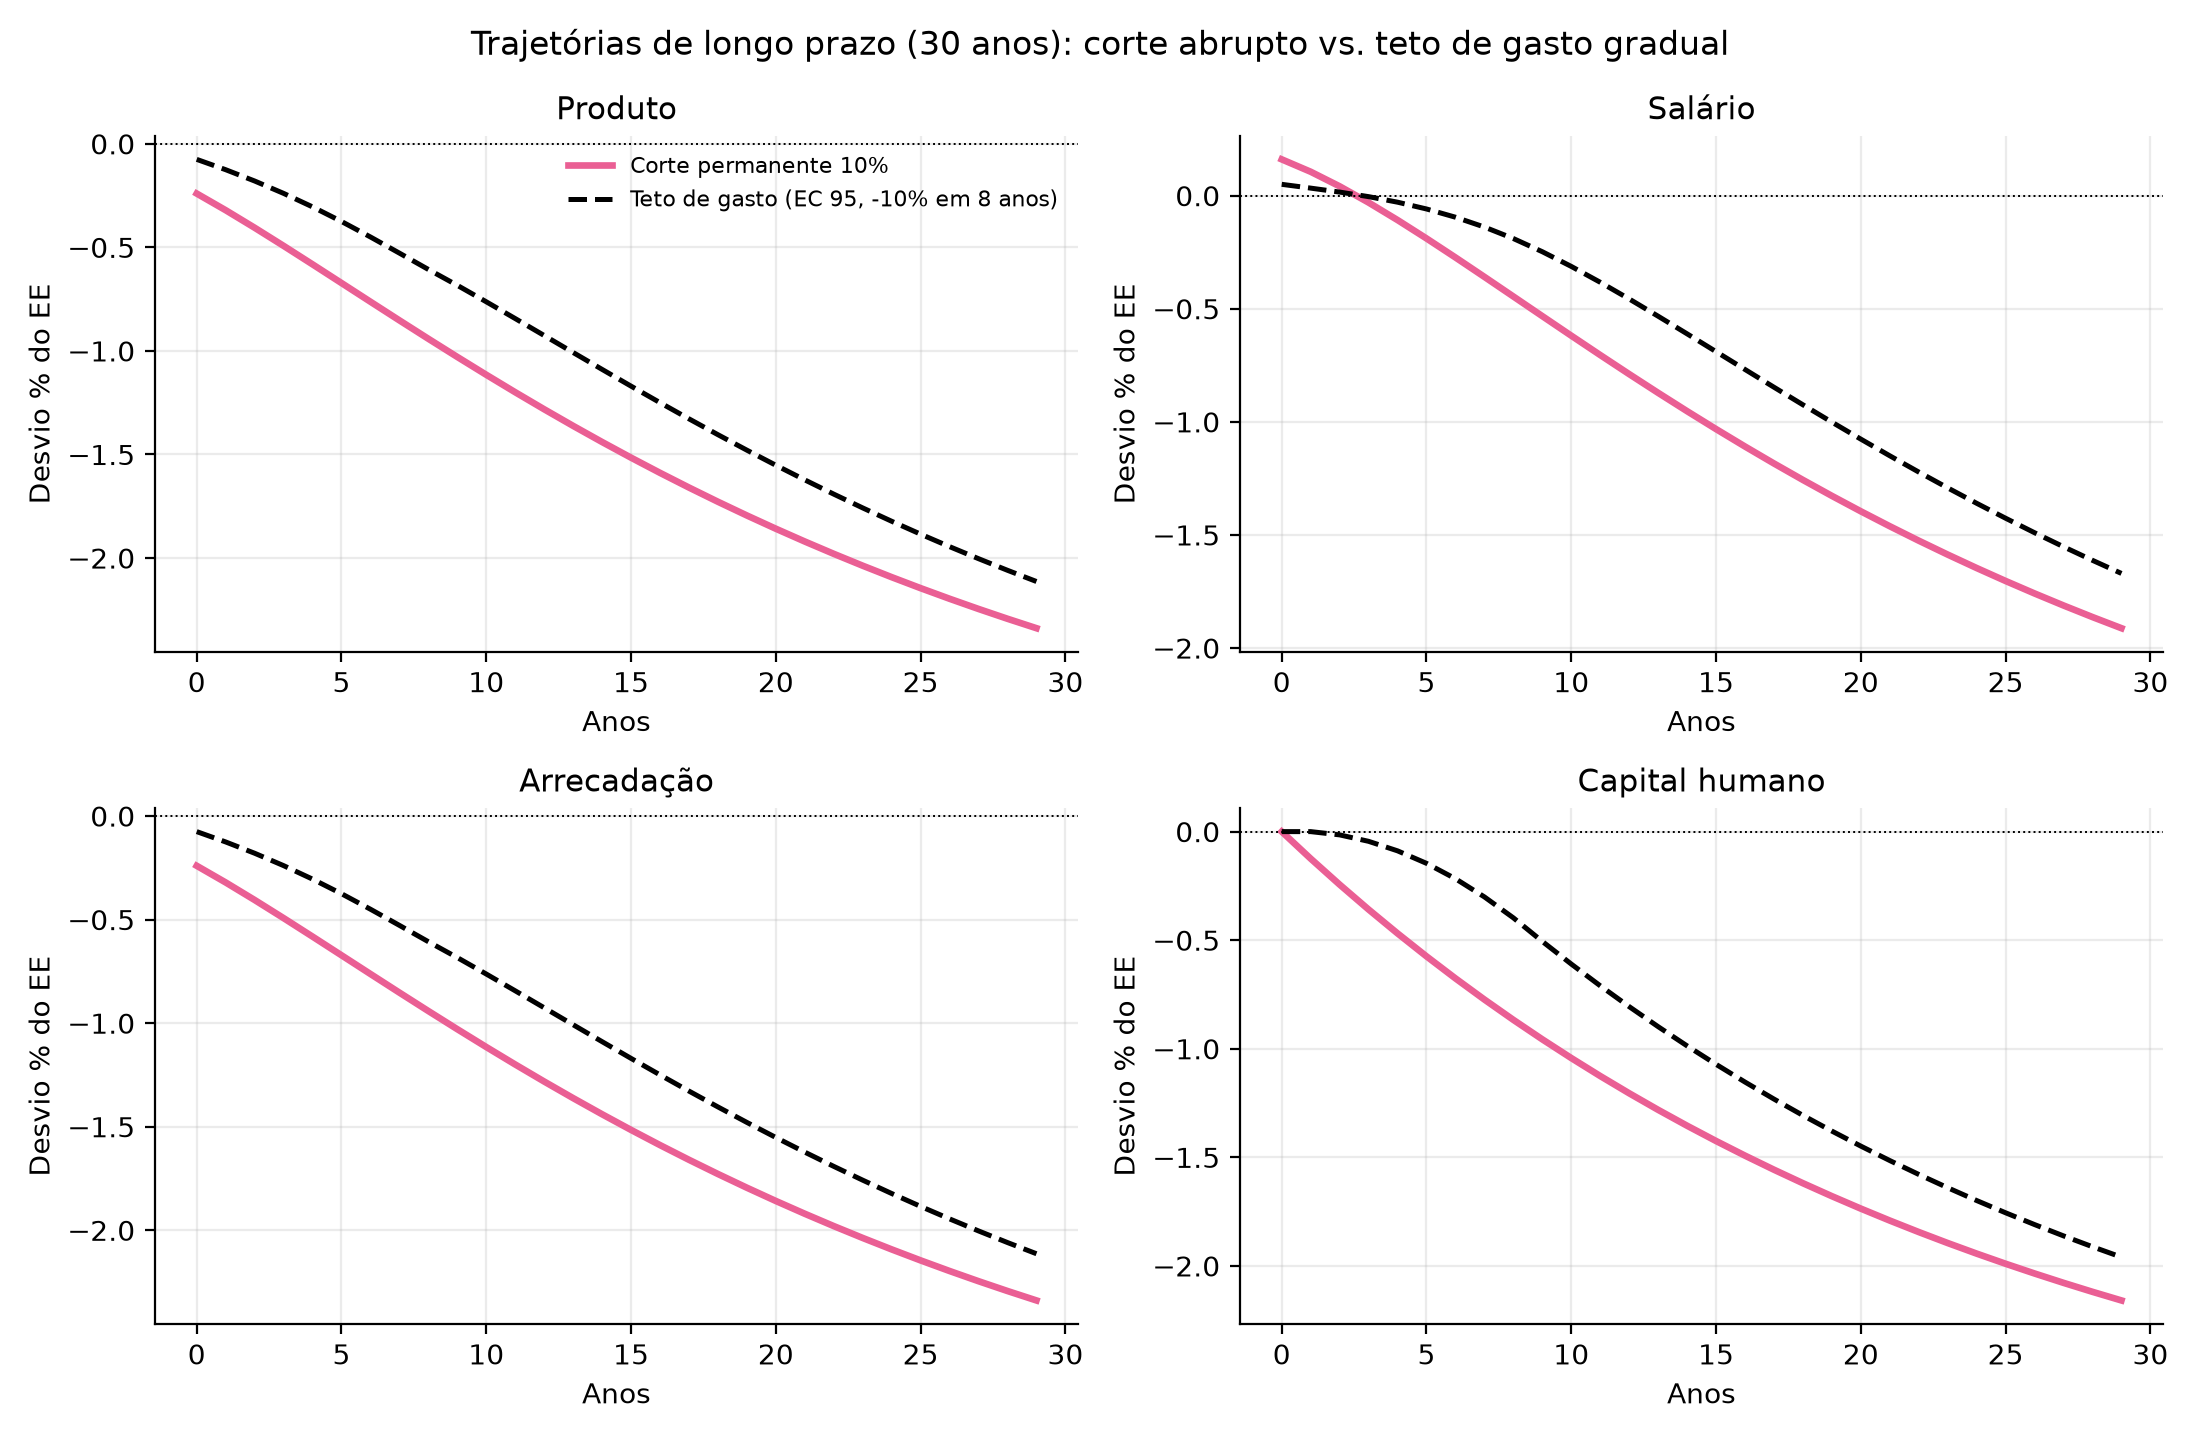
\includegraphics[width=\textwidth]{figures/trajetoria_30anos.png}
\caption{Trajet\'orias de 30 anos: corte abrupto de $10\%$ vs.\ teto de gasto gradual}
\label{fig:traj}
\fonte{Elabora\c{c}\~ao pr\'opria.}
\end{figure}

% =============================================================================
\section{Resultados II: o efeito Laffer din\^amico da educa\c{c}\~ao}\label{sec:laffer}
% =============================================================================
Ancorando o modelo em um PIB de R\$ $10{,}9$ trilh\~oes e um gasto p\'ublico em educa\c{c}\~ao de $5\%$ do PIB, traduzem-se as perdas em reais. A Tabela~\ref{tab:fisc} \'e o cerne do artigo. Para um corte de $10\%$, a economia acumulada em valor presente de 10 anos \'e de R\$ $457$ bilh\~oes, mas a perda de arrecada\c{c}\~ao consome $40\%$ desse valor; em 30 anos, a eros\~ao chega a $78\%$. A Figura~\ref{fig:fisc} mostra que, em fluxos n\~ao descontados, a perda acumulada de arrecada\c{c}\~ao \emph{ultrapassa} a economia por volta do ano 33 (\emph{break-even}): dali em diante, o corte \'e fiscalmente autodestrutivo.

\begin{table}[H]
\centering
\caption{Custo fiscal do corte em educa\c{c}\~ao (valor presente, R\$ bilh\~oes)}
\label{tab:fisc}
\small
\begin{tabular}{lrrrrr}
\toprule
Corte & Horizonte & Economia (VP) & Perda arrec.\ (VP) & Líquido (VP) & \% erodido \\
 & (anos) & R\$ bi & R\$ bi & R\$ bi & \\
\midrule
1\% & 10 & 45,7 & 17,9 & 27,8 & 39,2\% \\
1\% & 20 & 76,0 & 46,2 & 29,9 & 60,7\% \\
1\% & 30 & 96,2 & 73,3 & 22,9 & 76,2\% \\
\midrule
5\% & 10 & 228,3 & 89,9 & 138,4 & 39,4\% \\
5\% & 20 & 380,1 & 232,6 & 147,5 & 61,2\% \\
5\% & 30 & 481,1 & 370,0 & 111,0 & 76,9\% \\
\midrule
10\% & 10 & 456,7 & 180,9 & 275,8 & 39,6\% \\
10\% & 20 & 760,3 & 470,1 & 290,2 & 61,8\% \\
10\% & 30 & 962,1 & 748,9 & 213,2 & 77,8\% \\
\midrule
25\% & 10 & 1.141,7 & 461,9 & 679,8 & 40,5\% \\
25\% & 20 & 1.900,7 & 1.216,1 & 684,5 & 64,0\% \\
25\% & 30 & 2.405,3 & 1.947,4 & 457,9 & 81,0\% \\
\midrule
\bottomrule
\end{tabular}

\fonte{Elabora\c{c}\~ao pr\'opria. ``\% erodido'' = perda de arrecada\c{c}\~ao / economia or\c{c}ament\'aria.}
\end{table}

\begin{figure}[H]
\centering
\begin{minipage}{0.55\textwidth}\centering
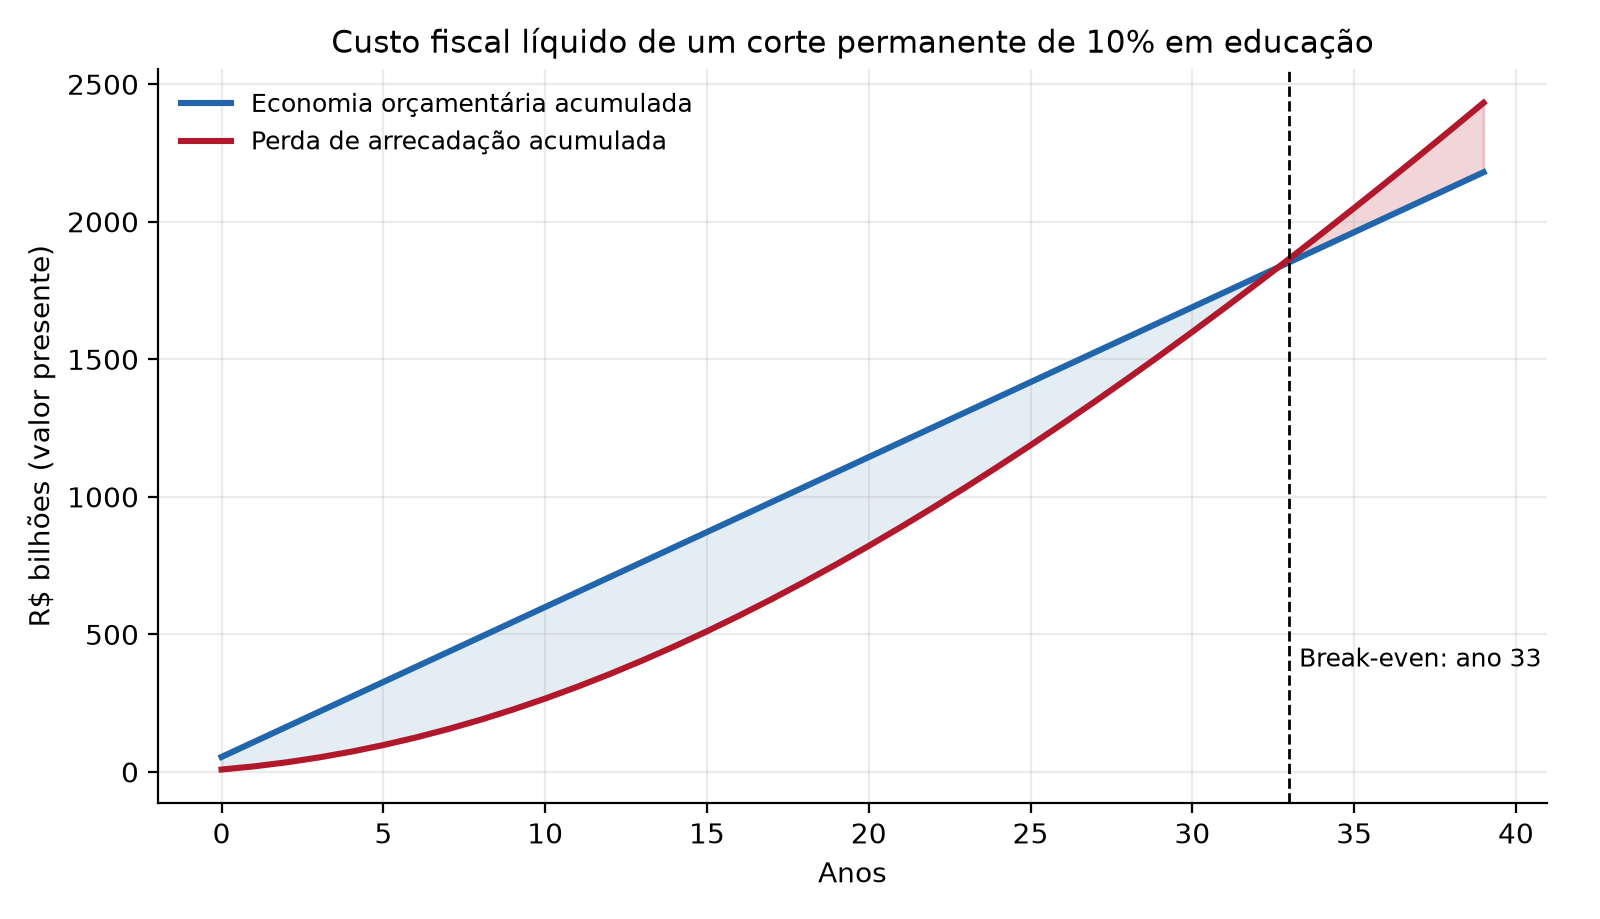
\includegraphics[width=\textwidth]{figures/custo_fiscal.png}
\end{minipage}\hfill
\begin{minipage}{0.43\textwidth}\centering
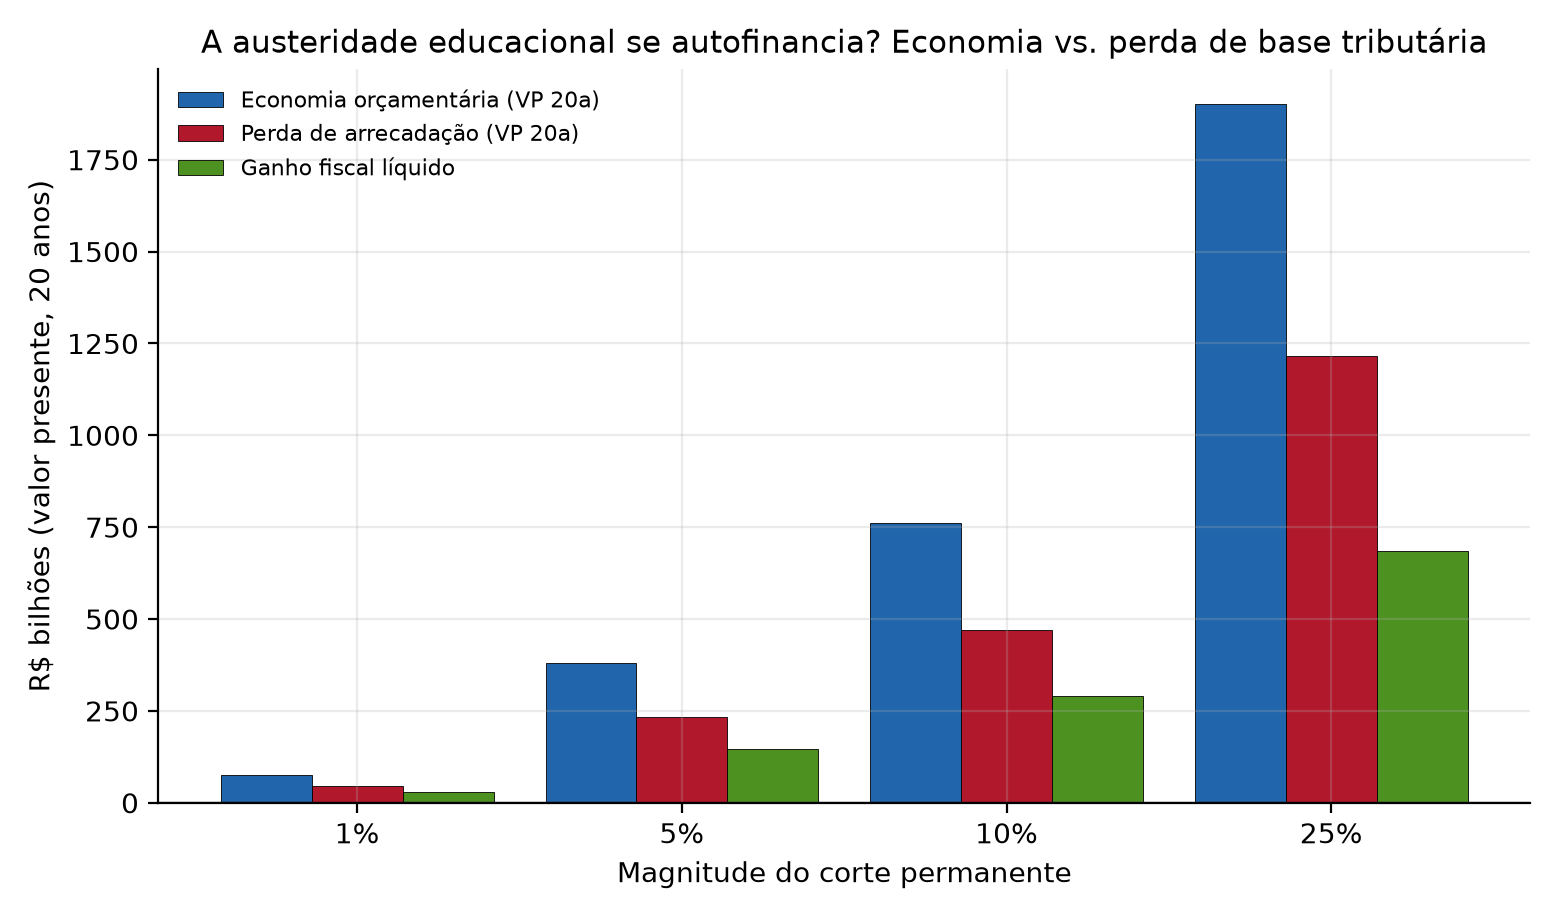
\includegraphics[width=\textwidth]{figures/custo_fiscal_barras.png}
\end{minipage}
\caption{Custo fiscal l\'iquido no tempo (corte de $10\%$, esq.) e economia vs.\ perda de arrecada\c{c}\~ao por magnitude (VP 20 anos, dir.)}
\label{fig:fisc}
\fonte{Elabora\c{c}\~ao pr\'opria.}
\end{figure}

\subsection{Um limiar de autofinanciamento}
Qu\~ao robusto \'e esse resultado \`a produtividade do gasto? A Figura~\ref{fig:laffer} e a Tabela~\ref{tab:laffer} variam o par\^ametro-chave $\phi$ para um corte de $10\%$. Quanto maior $\phi$, mais produtivo o gasto e maior a eros\~ao fiscal: o percentual erodido em 30 anos sobe de $54\%$ (para $\phi=0{,}15$) a mais de $100\%$ (para $\phi=0{,}45$), e o ano de \emph{break-even} cai de 95 para 23 anos. Existe, portanto, um \emph{limiar de autofinanciamento}: acima de $\phi\approx 0{,}45$, o ganho fiscal l\'iquido de 30 anos torna-se \emph{negativo} -- o corte perde dinheiro at\'e em valor presente. Como as estimativas de produtividade do capital p\'ublico frequentemente situam $\phi$ na faixa $0{,}2$--$0{,}4$ \citep{bomligthart2014}, o resultado qualitativo \'e forte: sob calibra\c{c}\~oes plaus\'iveis, a maior parte da economia or\c{c}ament\'aria \'e ilus\'oria.

\begin{figure}[H]
\centering
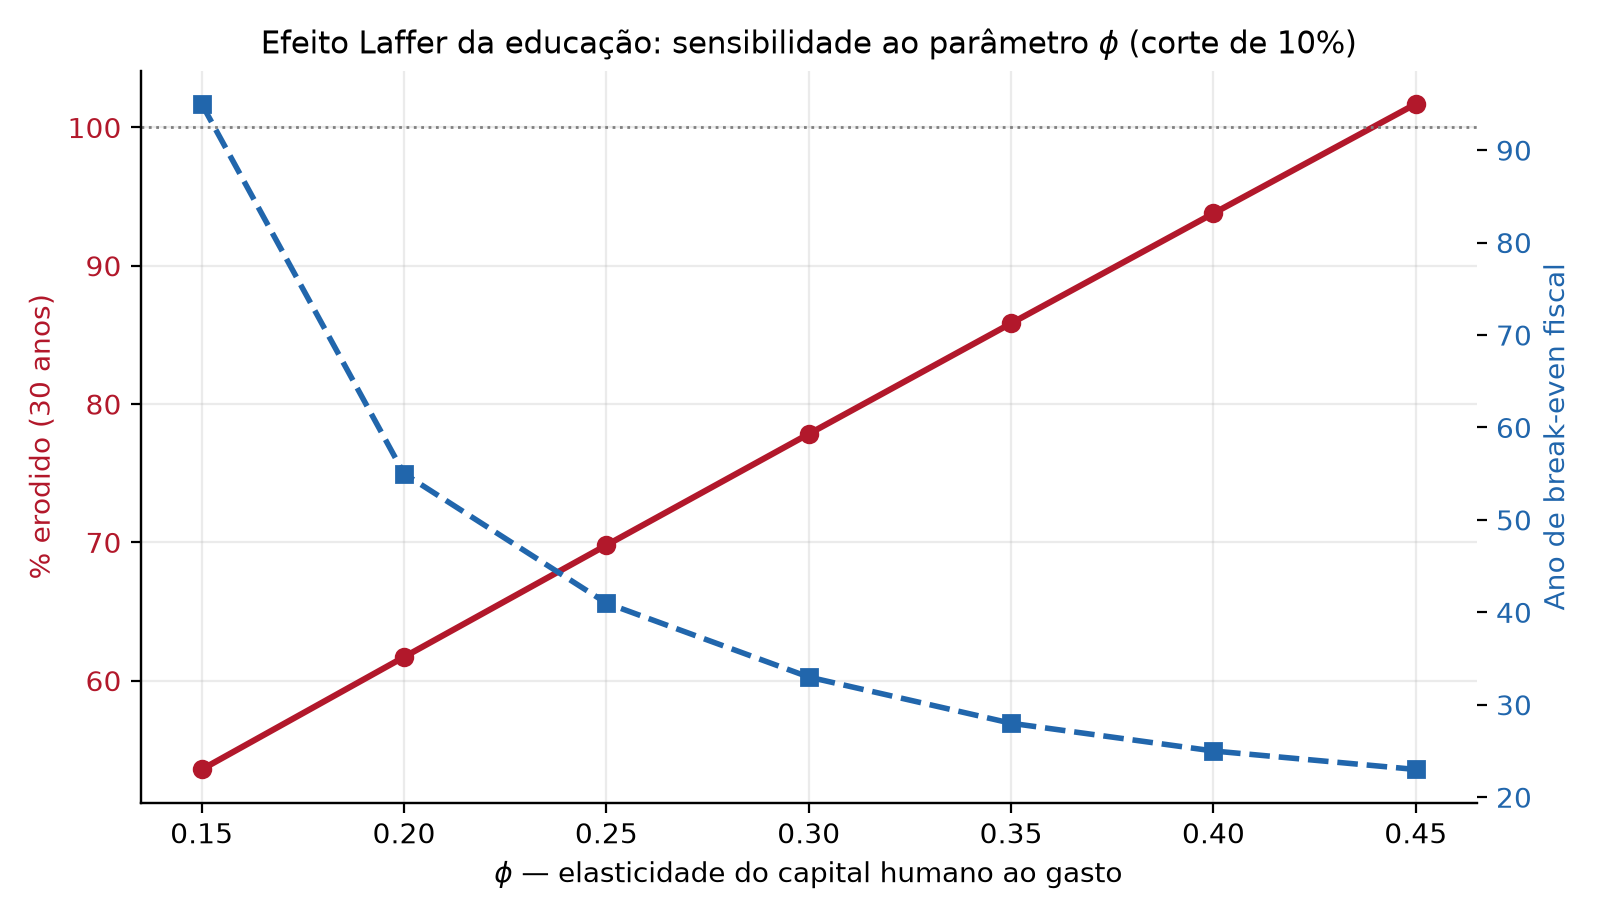
\includegraphics[width=0.82\textwidth]{figures/laffer_phi.png}
\caption{Efeito Laffer: sensibilidade ao par\^ametro $\phi$ (corte de $10\%$)}
\label{fig:laffer}
\fonte{Elabora\c{c}\~ao pr\'opria.}
\end{figure}

\begin{table}[H]
\centering
\caption{Custo fiscal l\'iquido em fun\c{c}\~ao de $\phi$ (corte permanente de $10\%$)}
\label{tab:laffer}
\small
\begin{tabular}{lrrrr}
\toprule
$\phi$ & $\Delta Y_{LP}$ (\%) & \% erodido 30a & Break-even (ano) & Líquido 30a (R\$ bi) \\
\midrule
0,15 & -1,972 & 53,6\% & 95 & 446,6 \\
0,20 & -2,464 & 61,7\% & 55 & 368,4 \\
0,25 & -2,953 & 69,8\% & 41 & 290,6 \\
0,30 & -3,440 & 77,8\% & 33 & 213,2 \\
0,35 & -3,924 & 85,8\% & 28 & 136,3 \\
0,40 & -4,406 & 93,8\% & 25 & 59,7 \\
0,45 & -4,885 & 101,7\% & 23 & -16,4 \\
\bottomrule
\end{tabular}

\fonte{Elabora\c{c}\~ao pr\'opria. Valores negativos de ``L\'iquido'' indicam corte que perde dinheiro em VP.}
\end{table}

% =============================================================================
\section{Resultados III: bem-estar e multiplicadores}\label{sec:bem}
% =============================================================================
Al\'em do custo fiscal, o corte imp\~oe custo de bem-estar. A Tabela~\ref{tab:cen} reporta a varia\c{c}\~ao equivalente de consumo: de $0{,}08\%$ (corte de $1\%$) a $2{,}4\%$ do consumo permanente (corte de $25\%$). O \emph{multiplicador acumulado} do gasto educacional sobre o produto -- raz\~ao entre valores presentes de $\Delta Y$ e $\Delta G^e$ -- supera a unidade e cresce no horizonte (Figura~\ref{fig:bem}, dir.; Tabela~\ref{tab:mult}), atingindo $\approx 1{,}2$ em 10 anos: cada real cortado subtrai \emph{mais de um real} de produto ao longo do tempo, porque o gasto \'e produtivo, n\~ao mera transfer\^encia.

\begin{figure}[H]
\centering
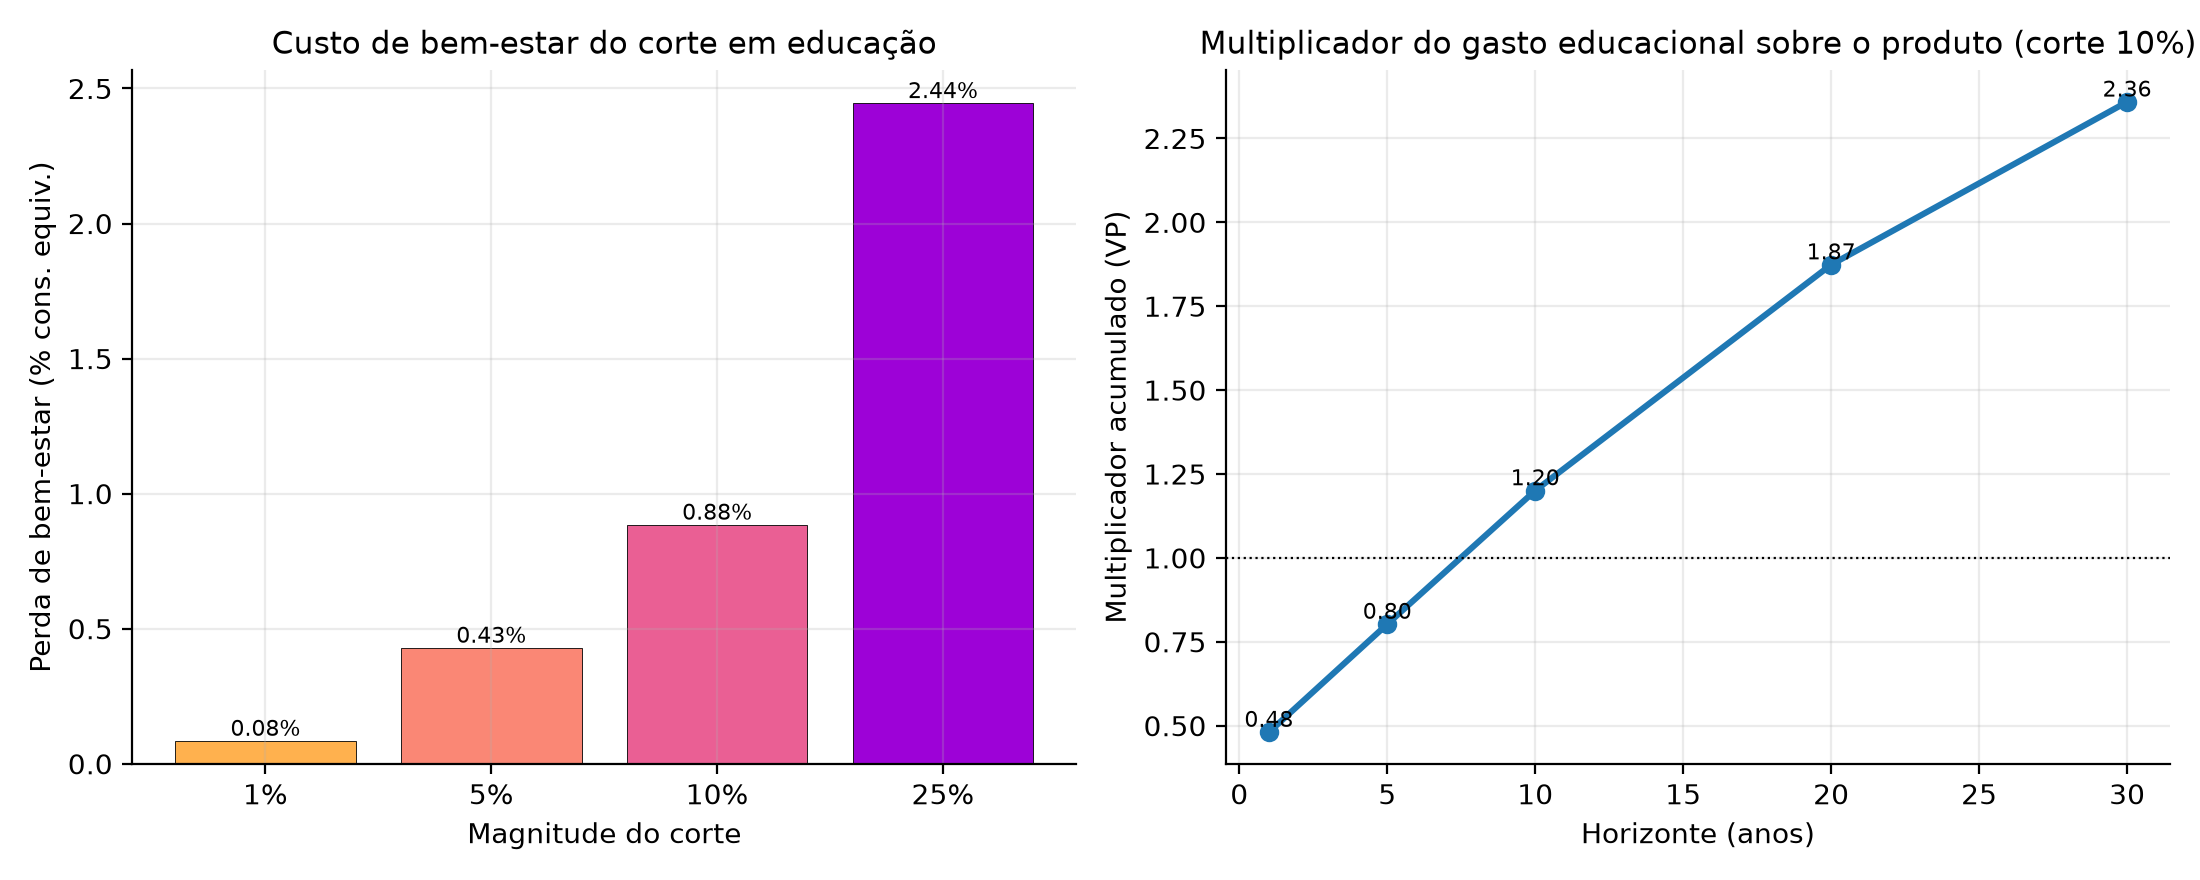
\includegraphics[width=\textwidth]{figures/bemestar_multiplicador.png}
\caption{Perda de bem-estar (esq.) e multiplicador acumulado do gasto educacional (dir.)}
\label{fig:bem}
\fonte{Elabora\c{c}\~ao pr\'opria.}
\end{figure}

\begin{table}[H]
\centering
\caption{Multiplicador do gasto educacional sobre o produto (por horizonte)}
\label{tab:mult}
\small
\begin{tabular}{lrrrrrr}
\toprule
Corte & Impacto & Cum.\ 1a & Cum.\ 5a & Cum.\ 10a & Cum.\ 20a & Cum.\ 30a \\
\midrule
1\% & 0,49 & 0,49 & 0,80 & 1,19 & 1,84 & 2,31 \\
5\% & 0,48 & 0,48 & 0,80 & 1,19 & 1,85 & 2,33 \\
10\% & 0,48 & 0,48 & 0,80 & 1,20 & 1,87 & 2,36 \\
25\% & 0,47 & 0,47 & 0,81 & 1,23 & 1,94 & 2,45 \\
\bottomrule
\end{tabular}

\fonte{Elabora\c{c}\~ao pr\'opria.}
\end{table}

% =============================================================================
\section{Robustez}
% =============================================================================
O resultado qualitativo (perdas em todas as vari\'aveis e eros\~ao fiscal) \'e invariante \`a persist\^encia do choque e \`a sua magnitude; a escala das perdas de longo prazo \'e governada por $\phi$, cuja sensibilidade foi mapeada na Se\c{c}\~ao~\ref{sec:laffer}. A ado\c{c}\~ao de estado estacion\'ario terminal end\'ogeno corrige um vi\'es de solu\c{c}\~oes que fixam o EE inicial. O estado estacion\'ario satisfaz as raz\~oes macroecon\^omicas usuais ($K/Y\approx 1{,}9$ ao ano; $L_{ss}\approx 0{,}23$). As limita\c{c}\~oes s\~ao a natureza calibrada e estilizada do modelo; uma vers\~ao estrutural estimaria par\^ametros por m\'etodos bayesianos \citep{smetswouters2007,fvrr2016} e incorporaria rigidezes nominais e heterogeneidade de agentes.

% =============================================================================
\section{Conclus\~ao}
% =============================================================================
Este artigo mostrou, em um DSGE fiscal com capital humano, que cortes no gasto p\'ublico em educa\c{c}\~ao geram perdas persistentes de produto e bem-estar e, sobretudo, \emph{corroem a pr\'opria base fiscal}. A resposta \`a pergunta do t\'itulo \'e negativa: a austeridade educacional n\~ao se autofinancia -- ao contr\'ario, em horizonte relevante torna-se autodestrutiva, com at\'e $78\%$ da economia or\c{c}ament\'aria revertida em 30 anos e um limiar de par\^ametro acima do qual o corte perde dinheiro at\'e em valor presente. A mensagem de pol\'itica \'e que regras fiscais que comprimem uniformemente a despesa educacional internalizam um custo fiscal futuro invis\'ivel \`a contabilidade de curto prazo. A agenda seguinte \'e a estima\c{c}\~ao estrutural do modelo e a incorpora\c{c}\~ao de d\'ivida p\'ublica e rigidezes.

\section*{Declara\c{c}\~ao sobre uso de IA generativa}
Este documento foi organizado e redigido com aux\'ilio de IA generativa a partir de c\'odigo, modelos e instru\c{c}\~oes do autor; a concep\c{c}\~ao, a valida\c{c}\~ao e a responsabilidade cient\'ifica s\~ao integralmente do autor.

\section*{Disponibilidade de dados e c\'odigo}
Todo o material para reprodu\c{c}\~ao -- base de dados, c\'odigo-fonte (Python e R), figuras e tabelas -- est\'a dispon\'ivel publicamente no reposit\'orio do projeto: \url{https://github.com/valbergregory/artigo-dsge-educacao} (vers\~ao arquivada com DOI no Zenodo: \texttt{10.5281/zenodo.XXXXXXX}). O reposit\'orio cont\'em \texttt{code/} (scripts \texttt{01}--\texttt{05} em Python e portes \texttt{03}--\texttt{04} em R para o RStudio), \texttt{paper/} (fontes LaTeX, figuras e tabelas) e \texttt{run\_all.py} (pipeline completo). Os valores monet\'arios s\~ao deflacionados pelo IPCA. Por padr\~ao o c\'odigo usa uma base calibrada realista; a coleta das s\'eries oficiais (Banco Central/SGS para o IPCA; SIDRA/IBGE para PIB e rendimento; SICONFI/FINBRA para finan\c{c}as estaduais; SIOP/Tesouro para o gasto federal em educa\c{c}\~ao) \'e ativada com \texttt{use\_api = TRUE}. C\'odigo sob licen\c{c}a MIT; texto sob CC-BY 4.0.

\bibliography{referencias}

\appendix
\section{Estado estacion\'ario terminal end\'ogeno}\label{ap:ss}
No EE, a Euler implica $K/Y=\alpha/\tilde{R}$ com $\tilde{R}=(1/\beta-1+\delta_k)/(1-\tau)$. Para um n\'ivel fixo de gasto $G^e$, o EE tem solu\c{c}\~ao fechada: $H=A(G^e)^\phi/\delta_h$; $Y=B\,H\,l$ com $B=(\alpha/\tilde{R})^{\alpha/(1-\alpha)}$; e
\[
l = \frac{(1-\tau)(1-\alpha)B\,H + \theta\,G^e}{B\,H\,[\theta(1-\delta_k K/Y) + (1-\tau)(1-\alpha)]}.
\]
Com a calibra\c{c}\~ao da Tabela~\ref{tab:par} e $G^e=G^e_{ss}$, recupera-se o EE base ($K/Y\approx1{,}89$, $L_{ss}\approx0{,}23$, $g_e=0{,}05$); um corte permanente de $1\%$ reduz $H$ em $\phi\%=0{,}30\%$.

\end{document}
